% ========== MUFLONFÅR ==========
\begin{frame}{%
  \begin{minipage}[c]{0.30\textwidth}
    Muflonfår
  \end{minipage}%
  \hfill
  \begin{minipage}[c]{0.45\textwidth}
    \footnotesize
    \textbf{Jagttid:} 1.\ oktober -- 31.\ januar
  \end{minipage}%
  \hfill
  \begin{minipage}[c]{0.15\textwidth}
    \noindent\raggedleft
    
\includegraphics[width=0.5cm, height=0.5cm, keepaspectratio]{Billeder/Ikoner/star.png}
  \end{minipage}%
}
  \vspace{0.25em}
  \begin{columns}[T]
    \column{0.45\textwidth}
    \setlength{\parskip}{0.4em}
    \tiny
    \RaggedRight
    \textbf{\textit{Ovis musimon}} – hunnen hos muflon. Lever ofte i flok med lam og unge dyr. \par
    \textbf{Udseende:}\\
    \quad – Ingen eller kun korte horn \\
    \quad – Mindre end vædderen \\
    \quad – Rustrød til mørk pels, typisk uden de store lyse saddelpletter \\
    \quad – Kraftig krop og forholdsvis spinkle ben \par
    \textbf{Levesteder:} Åbne sletter, overdrev, hede og skovbryn. Trives dårligt i tæt skov. \par
    \textbf{Føde:} Græs og urter. Om vinteren også bark og stedsegrøn vegetation. \par
    \textbf{Udbredelse:} Enkelte småøer og udslip fra dyrehaver. \par
   % \textbf{Parring/brunst:} Efterår. \par
   % \textbf{Forplantning:}\\
    %\quad – \textbf{Kønsmoden:} Ca. 2 år \\
    %\quad – \textbf{Mono/polygam:} Polygam \\
    %\quad – \textbf{Bestandsomsætning:} Langsom \\
    %\quad – \textbf{Kuld:} 1 lam, sjældent 2
    \column{0.52\textwidth}
    \centering
    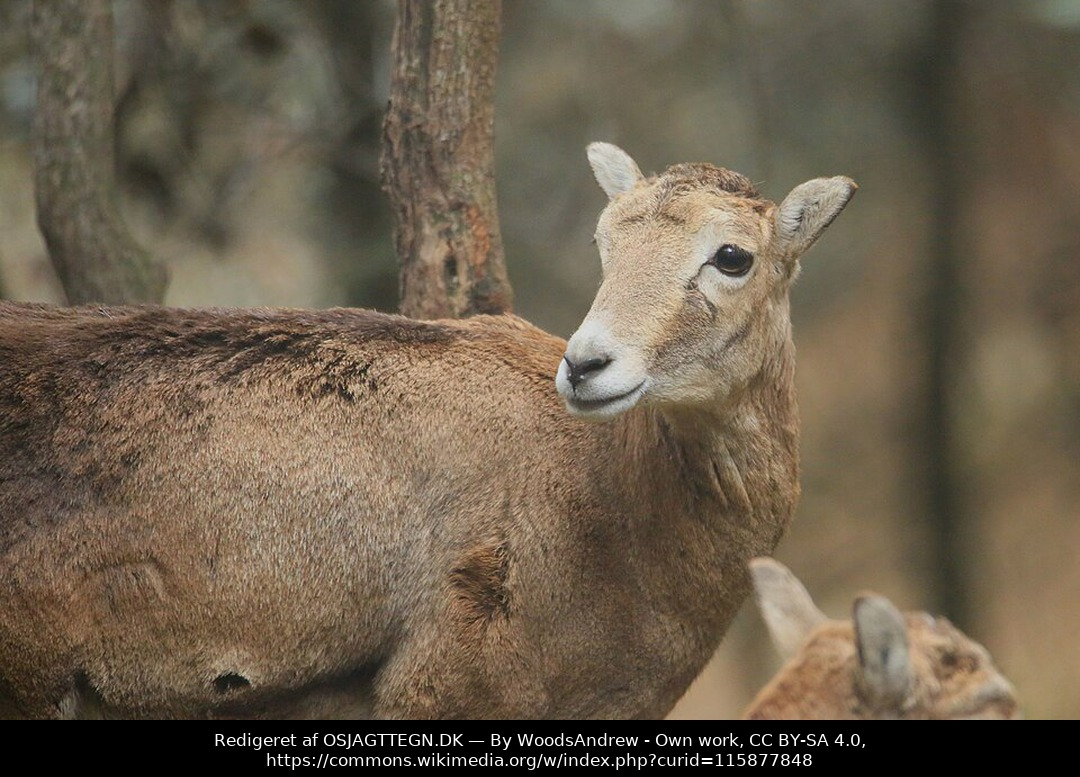
\includegraphics[width=\linewidth, height=7.2cm, keepaspectratio]{Billeder/Dyr/Pattedyr/hovdyr/muflon/muflon-female-01.jpg}
  \end{columns}
\end{frame}